\chapter{Návrh riešenia}
\label{kap:navrh} % id kapitoly pre prikaz ref


\section{Návrh ontológie}

\begin{figure}[h]
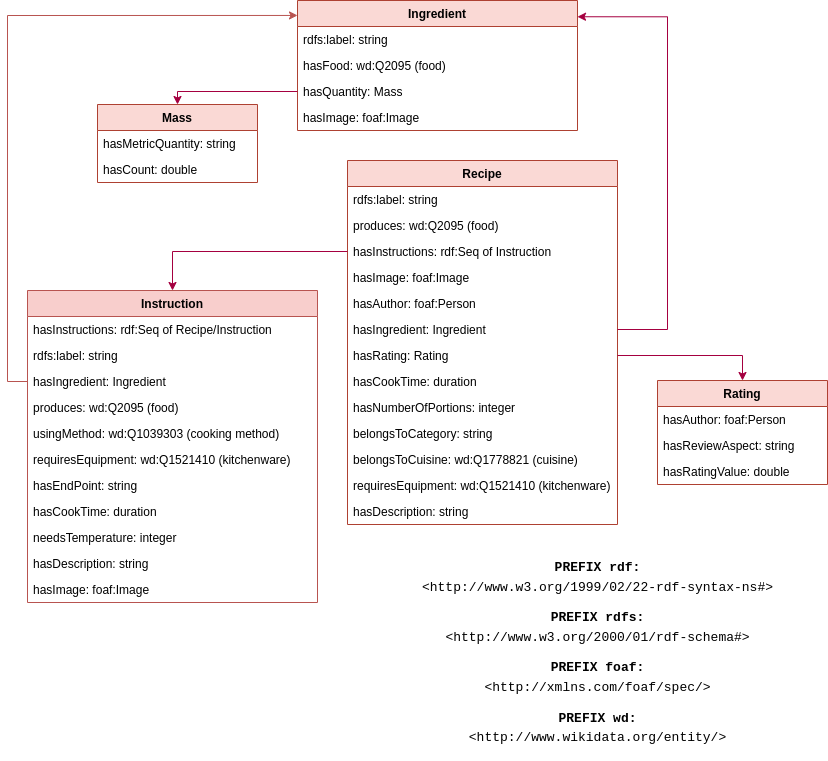
\includegraphics[width=\textwidth]{images/ontology}
\caption{Grafické vyjadrenie návrhu ontológie o receptoch}
\label{ontology}
\end{figure}

\subsection{Protégé}
Na vytvorenie ontológie sme využili Protégé, ktorý je možné stiahnuť na stránke \href{https://protege.stanford.edu/}{https://protege.stanford.edu/}. Protégé poskytuje grafické používateľské rozhranie, je to voľne dostupný editor ontológií a framework pre budovanie inteligentných systémov. Umožňuje modelovať triedy, predikáty, či vytvárať obmedzenia na jednotlivé predikáty. Následne je možné uložiť takto vytvorenú ontológiu v niektorej zo syntaxí pre jazyk OWL. Pri tvorbe našej ontológie sme využívali túto základnú funkcionalitu.

\subsection{Existujúca ontológia}
	Naša ontológia nadväzuje na ontológiu o receptoch v minuloročnej bakalárskej práci \cite{bakalarka}. Hlavnou úlohou bolo rozšíriť pôvodnú ontológiu o triedu, respektíve triedy, ktoré budú reprezentovať jednotlivé kroky (inštrukcie) v postupe receptu, keďže predtým bol postup iba pole reťazcov. V priebehu tvorby ontológie však došlo aj k ďalším menším zmenám v existujúcich triedach. Zároveň boli z pôvodnej ontológie odstránené triedy ingredientList a Food. Trieda ingredientList iba zapuzdrovala všetky ingrediencie patriace ku konkrétnemu receptu a trieda Food, ktorá vyjadrovala už existujúcu triedu a v našom prípade nebolo potrebné k nej pridávať žiaden ďalší predikát.
	
\subsection{Navrhnutá ontológia}
Nižšie je popísaná ontológia podľa obr. \ref{ontology}. Pri popisovaní ontológie je v zátvorkách uvedený presný názov predikátu tak, ako sa nachádza v ontológií a v jej grafickom vyjadrení na obr. \ref{ontology}. V pravom dolnom rohu obr. \ref{ontology} sú uvedené využité prefixy v prípade, že trieda alebo predikát boli prevzaté z už existujúceho slovníka. 
	
\subsubsection{Popis tried existujúcich v predchádzajúcej ontológií}
	Hlavnou triedou je trieda Recipe, ktorá popisuje recept ako celok. Každý recept môže mať priradený obrázok (hasImage), názov vytváraného receptu zrozumiteľný pre používateľa (rdfs:label), autora (hasAuthor), čas potrebný na prípravu (hasCookTime), počet porcií, ktoré daný recept vytvára (hasNumberOfPortions), stručný popis, ktorý však ešte nepatrí k postupu (hasDescription) a môžnosť zaradiť recept do nejakej kategórie (belongsToCategory), pričom tento predikát môže byť použitý opakovane v prípade, že recept patrí do viacerých kategórií. Ďalšími predikátmi sú príslušnosť k nejakej národnej kuchyni (belongsToCuisine), požadované kuchynské potreby (requiresEquipment), hodnotenia daného receptu inými používateľmi (hasRating). V tom prípade je objektom inštancia triedy Rating, pričom každé hodnotenie má autora(hasAuthor) a môže obsahovať nejaký slovný komentár (hasReviewAspect) alebo číselne vyjadrenú spokojnosť s receptom (hasRatingValue). Každý recept vytvára nejaké jedlo, ktoré sa v niektorých prípadoch môže použiť ako ingrediencia v inom recepte, a preto bolo potrebné recept zaradiť aj do triedy Food (produces).
	
	Predikát umožňujúci priradzovať k danému receptu ingrediencie (hasIngredient) spája triedu Recipe s triedou Ingredient. Každá ingrediencia môže mať názov zrozumiteľný pre používateľa (rdfs:label), obrázok (hasImage), jednotku merania (hasMetricQuantity), množstvo (hasCount), pričom posledné 2 spomenuté predikáty patria triede Mass. Každá ingrediencia je nejaké už existujúce jedlo (hasFood).
	
\subsubsection{Popis triedy Instruction}
	Každý recept musí mať nejaký postup (hasInstructions). Objektom tohto predikátu je kontainer Alt, ktorý sa používa v prípadoch, kedy si používateľ môže vybrať jednu z možností, ktoré kontainer obsahuje. V tomto prípade je možné do kontainera pridávať inštancie triedy Recipe, keďže k jednému jedlu existuje viacero receptov a takýmto spôsobom sa na nich odkážeme, alebo inštancie triedy Instruction, ak vytvárame náš vlastný postup. 
	
	Pri definovaní krokov v postupe receptu sme uvažovali nad viacerými možnosťami ako ich vytvárať. Plánovali sme oddeľovať triedu Description, Stage a Step, vďaka ktorým by sa dal recept pekne rozčleniť. Avšak nie každý recept má takúto štruktúru a pri iných typoch receptov by boli častokrát zbytočné triedy Stage, či Description. V prípade samotného kroku sme uvažovali nad tým, že bude obsahovať triedu Activity, ktorá presne popíše, ktorú surovinu, akým spôsobom, a za akých podmienok bude spracovávať. Toto by síce dokonale rozobralo každý krok receptu, avšak praktické využitie takto podrobnej ontológie by bolo príliš náročné. 
	
	Rozhodli sme sa preto pre možnosť vytvoriť jedinú triedu Instruction. Inštrukcia môže zaobaľovať celú postupnosť krokov k receptu, môže vyjadrovať nejakú časť krokov, ktoré tvoria samostatnú časť jedla, napr. v prípade koláča to je inštrukcia na vytvorenie plnky, cesta, či polevy, alebo môže inštrukcia vyjadrovať jediný krok. Využitie triedy bude teda závisieť od toho, ako bude vyzerať postup k receptu. Práve kvôli rôznorodosti postupov sme museli vytvoriť dostatočne všeobecnú triedu, aby mohla umožniť rovnako ľahko vytvoriť recept s jedným krokom, ako aj recept s pomerne zložitým postupom, v ktorom sú isté časti receptu oddelené do samostatných celkov. Používateľovi je umožnené priradiť techniku prípravy, ktorú je potrebné využiť pri danom kroku (usingMethod), napr. vyprážanie, pečenie, možnosť priradiť obrázok (hasImage), názov (rdfs:label), teplotu, pri ktorej má byť daná inštrukcia vykonávaná (needsTemperature), požadované kuchynské potreby (requiresEquipment), či potraviny spracovávané v danej časti receptu (hasIngredient).  Trieda Instruction ďalej umožňuje vyjadriť čas potrebný na vykonanie nejakého kroku (hasCookTime). V niektorých prípadoch je trvanie kroku vyjadrené slovne, napr. pečieme, kým nezhnedne, vtedy použijeme predikát, ktorý vyjadruje práve prechod ingrediencie do nejakého finálneho stavu (hasEndPoint). Ak ide o skupinu krokov, ktoré vytvárajú celý postup k receptu alebo časť receptu, napr. prípravu cesta pri pečení koláča, využijeme predikát hasInstructions. Ten ako objekt obsahuje sekvenciu ďalších inštrukcií, alebo receptov, v prípade, že by sme sa v nejakej časti receptu chceli odkázať na už existujúci recept. Trieda rdf:Seq nám umožňuje ukladať prvky tak, aby sme poznali poradie, v ktorom sme ich pridávali. Ak chceme popisovať už koncový krok, ktorý sa skladá iba zo slovného popisu a ďalej sa nečlení, využijeme predikát hasDescription. V prípade, že nejaká inštukcia vytvára jedlo, môžeme využiť predikát produces.
 
\section{Funkcionalita systému}
V tejto podkapitole popisujeme funkcionalitu systému. Ide o prehľad toho, čo používateľ môže využívať v prípade, že túto webovú aplikáciu navštívi.
\begin{enumerate}
\item \textbf{Registrácia používateľa} - Používateľ má možnosť sa zaregistrovať vyplnením formulára, kde je nutné uviesť meno, priezvisko a email. 
\item \textbf{Prihlásenie používateľa} - Po prihlásení môže používateľ vytvárať nové recepty a hodnotiť iné recepty.
\item \textbf{Možnosť, aj pre neprihláseného používateľa, pridať nové:}

\begin{itemize}
\item \textbf{ingrediencie}
\item \textbf{národné kuchyne}
\item \textbf{kuchynské potreby}
\item \textbf{spôsoby prípravy jedla}
\end{itemize} 

V prípade, že používateľ pokladá za potrebné pridať novú položku v niektorej  z vyššie uvedených kategórií, môže tak urobiť prostrednístvom vyplnenia formulára. (Možné pridať iba ingrediencie, o ktorých informácie sa nachádzajú na DBpedii, keďže následne by nebolo možné dohľadať informácie.)

\item \textbf{Zobrazenie receptu} - Každý používateľ, prihlásený aj neprihlásený, si môže zobraziť podrobnosti o recepte, ktoré autor receptu pri vytváraní zadal. V prípade, že autor niektoré polia formulára pri vytváraní nevyplnil, bude táto položka označená ako "Neuvedené". Pri každom recepte sa budú zobrazovať rovnaké, respektíve podobné recepty, na základe receptov, ktoré autor uviedol pri vytváraní receptu. 
\item \textbf{Pridanie vlastného receptu} - Každý prihlásený používateľ má možnosť vytvoriť vlastný recept. Povinnými poliami pre vytvorenie receptu sú názov, aspoň jedna ingrediencia, pri ktorej je potrebné uviesť množstvo a jednotku merania, a aspoň jeden krok v postupe. Ďalej je možné uviesť popis receptu, počet porcií, čas potrebný na prípravu, vybrať z kategórií a kuchýň do ktorých recept patrí, kuchynské potreby nutné na prípravu a fotografiu, ktorá v prípade nevyplnenia používateľom bude defaul.png. Pri vypĺňaní postupu receptu je možné uvádzať kroky aj podkroky. Ak má krok podkroky, v tom prípade je nutné uviesť názov celého kroku. Používateľ má možnosť uviesť pri jednotlivých krokoch a podkrokoch aj ingrediencie, spôsoby prípravy, kuchynské potreby, čas alebo popis stavu, v ktorom daný krok,respektíve podkrok končí, teplotu alebo fotografiu.
\item \textbf{Úprava ľubovoľného receptu, aj v prípade receptu iného používateľa} - Jednotlivé časti receptu môže používateľ upraviť po kliknutí na tlačidlo Edit, ktoré sa nachádza pri jednotlivých častiach receptu. V tom prípade sa používateľovi upravovaná časť receptu zobrazí v takej forme ako keď je vytváraná, avšak všetky polia budú predvyplnené. Ak po úprave ostanú vyplnené povinné polia, úprava sa bude považovať za úspešnú. Používateľ, ktorý recept vytvoril dostane upozornenie, že recept bol pozmenený. Všetkým používateľom sa v čase medzi úpravou a potvrdením úpravy zobrazuje aktualizovaný recept. Pôvodná verzia, ktorú používateľ vytvoril je však uchovaná a v prípade, že používateľ so zmenami nesúhlasí sa k nej môže vrátiť.
\item \textbf{Pridanie ďalších receptov vytvárajúcich rovnaké, respektíve podobné jedlo} - Pri vytváraní receptu má používateľ možnosť zadať recept, ktorý sa nachádza na stránke a vytvára rovnaké jedlo. Pridávať rovnaké recepty môžu aj ďalší používatelia bez toho, aby to autor receptu musel následne schvaľovať.
\item \textbf{Pridanie komentára alebo hodnotenia receptu} - Prihlásený používateľ má možnosť pridať hodnotenie receptu. Má možnosť pridávať aj slovný komentár k jednotlivým receptom.
\item \textbf{Možnosť, aj pre neprihláseného používateľa, vyhľadávať recepty podľa:} 

\begin{itemize}
\item \textbf{názvu} - Používateľ má možnosť vyhľadať recept zadaním jeho názvu. Vyhľadávané sú aj recepty, ktorých časť názvu sa zhoduje s tým, čo používateľ zadal.
\item \textbf{ingrediencií} - Používateľ má možnosť zvoliť si suroviny, teda ingrediencie, ktoré sú súčasťou jedla. Ak si zvolí viacero surovín, všetky zároveň budú musieť byť súčasťou jedál, ktoré sa mu zobrazia. Používateľovi je  umožnené, aby si zvolil aj ingrediencie, ktoré súčasťou jedla byť nemajú. V tom prípade sa v jedle nemôže nachádzať ani jedna z označených ingrediencií.
\item \textbf{autora} - Používateľ má možnosť si vyhľadať recepty od konkrétneho autora. V prípade, že autorov je zadaných viac, každý z vyhľadaných receptov patrí práve jednému z nich.
\item \textbf{národnej kuchyne} - Používateľ má možnosť zvoliť si jednu alebo viacero národných kuchýň, pričom každé jedlo bude patriť aspoň do jednej z nich.
\item \textbf{spôsobu prípravy jedla} - Používateľ má možnosť označiť jeden alebo viacero spôsobov prípravy, ktoré chce alebo nechce používať. Ak sú označené viaceré, do výberu sa dostávajú tie recepty, ktoré obsahujú aspoň jeden zo spôsobov, ktoré používateľ označil, že chce použiť, a zároveň ani jeden zo spôsobov, ktoré označil, že použiť nechce.
\item \textbf{kuchynských potrieb} - Používateľ má možnosť zvoliť si kuchynské potreby, ktoré chce, respektíve nechce použiť pri príprave jedla. V prípade výberu viacerých kuchynských potrieb, ktoré používateľ chce používať, budú vyhľadané recepty, v ktorých sú použité všetky potreby. V prípade výberu viacerých potrieb, ktoré používateľ nechce používať, budú odstránené z vyhľadávania tie, ktoré obsahujú aspoň jednu z označených potrieb.
\item \textbf{dĺžky prípravy}- Používateľ má možnosť zvoliť si interval dĺžky prípravy jedla, teda iba spodnú hranicu, iba hornú hranicu, alebo obidve naraz. 
\item \textbf{hodnotenia} - Používateľ má možnosť zvoliť si minimálne hodnotenie jedla, pričom zobrazované mu budú všetky recepty s hodnotením väčším alebo rovným.
\item \textbf{kategórie} - Používateľ má možnosť zvoliť si jednu alebo viacero kategórií jedál, pričom každé zo zobrazených jedál bude patriť aspoň do jednej z kategórií.
\end{itemize}

\item \textbf{Prepočítanie množstiev ingrediencií podľa počtu porcií} - Používateľ má možnosť zvoliť si počet osôb, pre ktoré chce daný recept pripravovať. Následne sú množstvá ingrediencií prepočítané. Táto možnosť nie je v prípade receptov, pri ktorých nie je uvedený počet porcií.
\item \textbf{Premena jednotiek, v ktorých zadávame ingrediencie} - Používateľ má možnosť pri recepte v zozname ingrediencií prepočítať jednotlivé množstvá ingrediencií na iné jednotky, ak nebude množstvo zadané popisne, teda napr. troška alebo štipka.
\item \textbf{Možnosť zistiť bližšie informácie o ingrediencií, jedle, kuchyni, spôsobe prípravy a vybranej kuchynskej potrebe} - Používateľ bude mať možnosť dozvedieť sa viac o veciach z uvedených kategórií. Bližšie informácie sa mu zobrazia po kliknutí na jej konkrétny názov. (Informácie budú získavané z DBpedie).
\end{enumerate}


